\section{System Management Operations}
\label{sec:management}

\subsection{Fault Tolerance}
\label{sec:resilience}

\subsubsection{Replicating Runtimes}
\label{sec:replicating-runtime}
\begin{figure}[!h]
\begin{subfigure}[t]{0.49\linewidth}
   \centering
   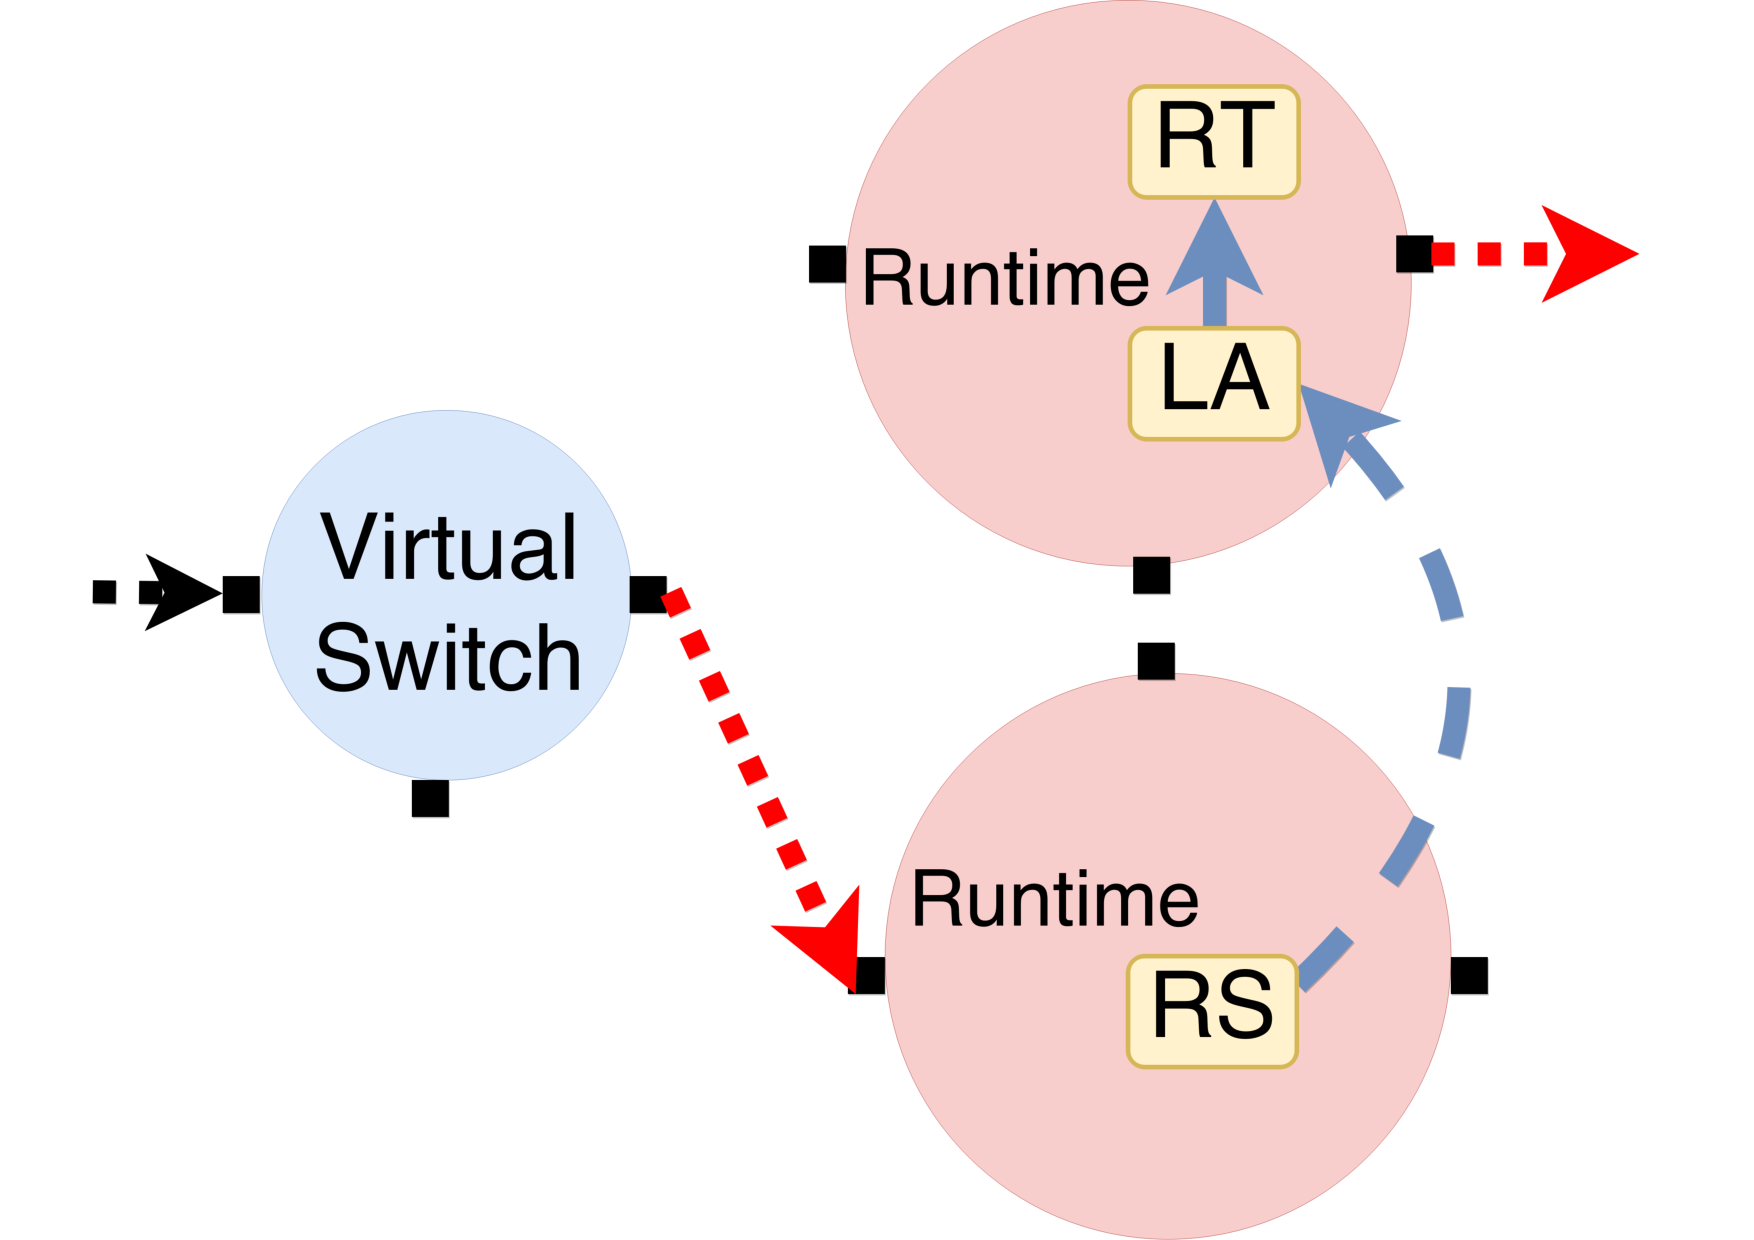
\includegraphics[width=\columnwidth]{chap-nfvactor/figure/nfactor-replication.pdf}
   \caption{Flow replication.}\label{fig:rep}
  \end{subfigure}
  \begin{subfigure}[t]{0.49\linewidth}
     \centering
     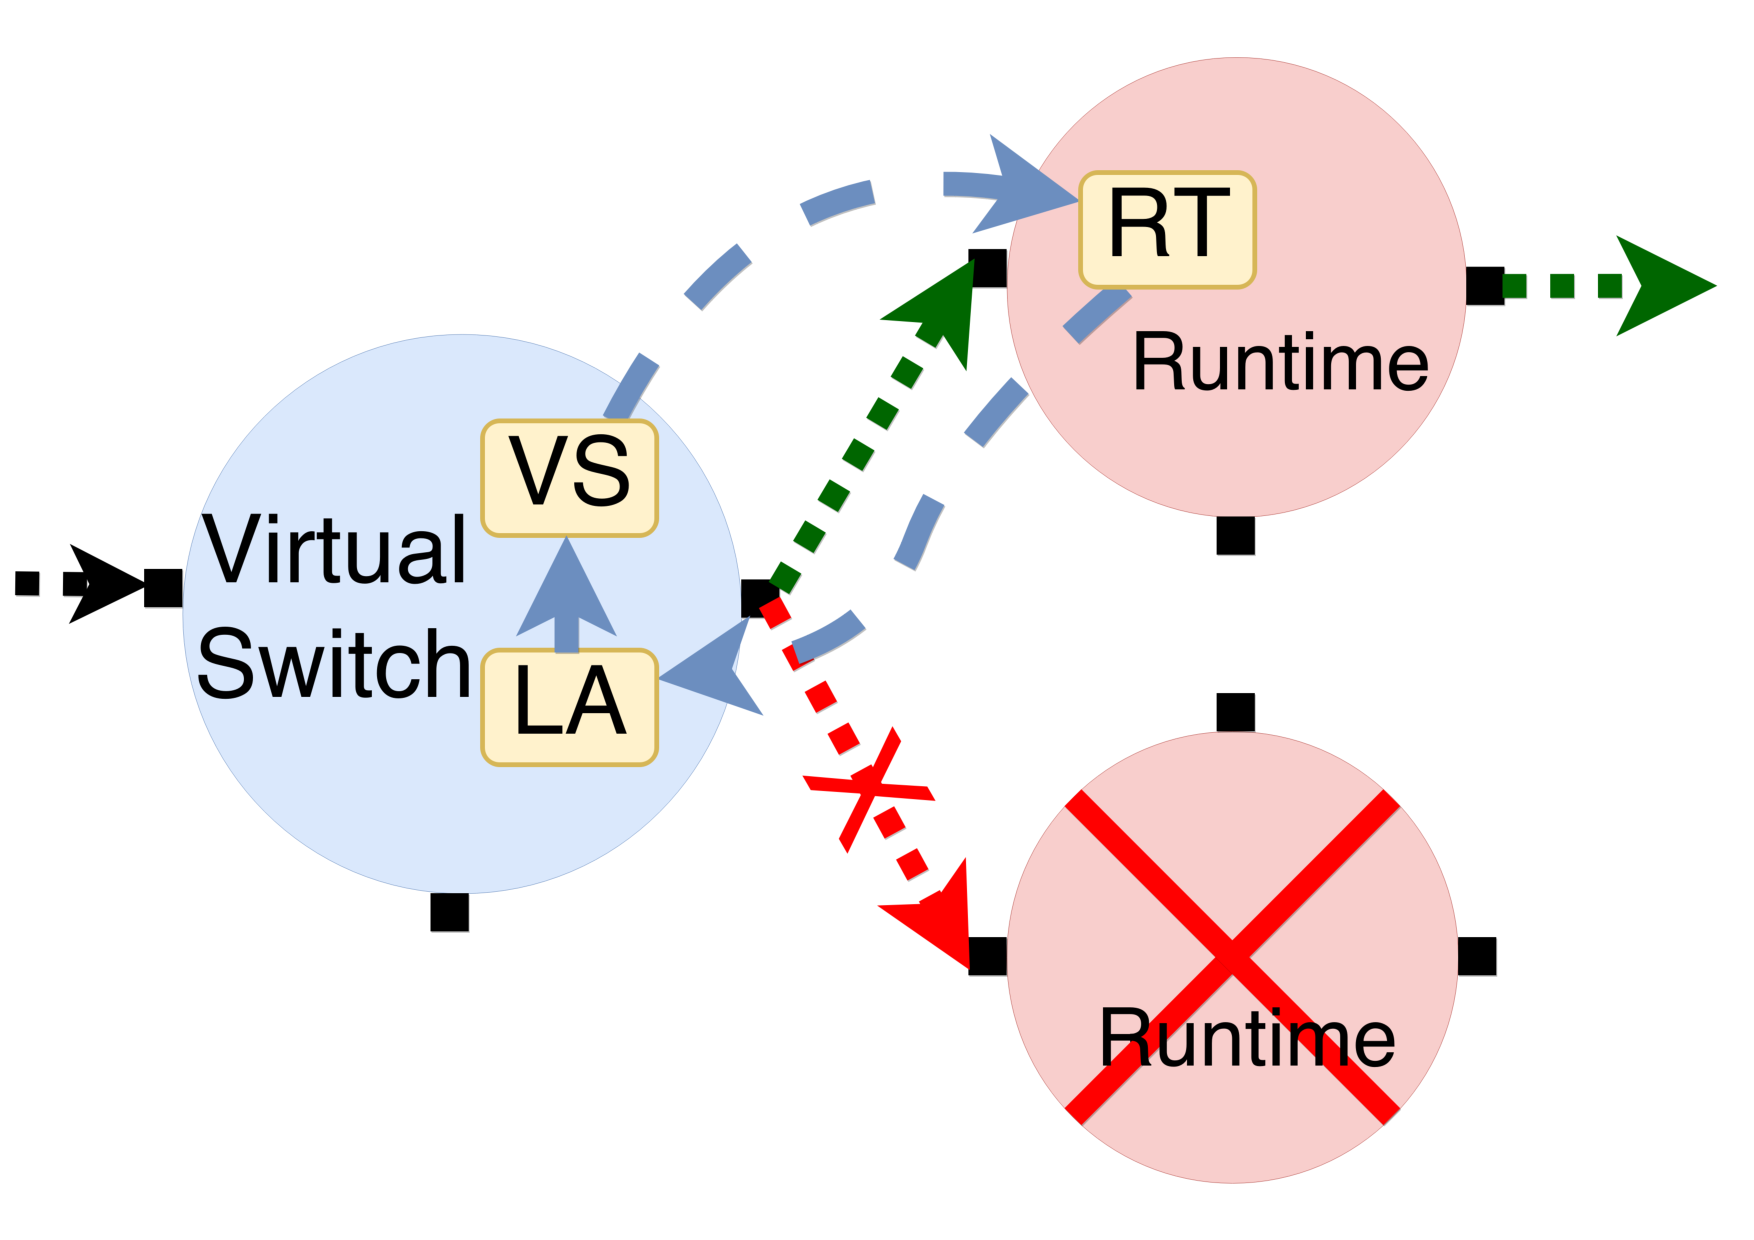
\includegraphics[width=\columnwidth]{chap-nfvactor/figure/nfactor-recover.pdf}
     \caption{Flow recover when the original runtime has failed.}\label{fig:recover}
    \end{subfigure}
 \caption{Flow replication and recovery: \textbf{RT} - replication target actor, \textbf{RS} - Replication source actor, \textbf{LA} - liaison actor, \textbf{VS} - virtual switch actor; \textbf{dotted line} - flow packets, \textbf{dashed line} - actor messages.)}
\label{fig:flow-rep}
\end{figure}

To perform lightweight runtime replication, we leverage the actor abstraction and state separation. In a runtime, important states associated with a flow are stored by the flow actor. The runtime can replicate each flow actor independently without check-pointing the entire container image \cite{sherry2015rollback, rajagopalan2013pico}. While achieving good throughput and fast flow recovery, this replication strategy also improves the packet processing delay and has good scalability, as each flow actor can replicate itself on another runtime without the need of dedicated back-up servers.

The detailed flow replication process is illustrated in Fig.~\ref{fig:flow-rep}. When a runtime is launched, the coordinator sends a list of runtimes in the same cluster to its liaison actor via RPC $set\_replicas(runtime\_id\_list)$. When a flow actor is created on the runtime, it acquires its replication target runtime from the liaison actor, selected in a round-robin fashion among all available runtimes received from the coordinator.

When a flow actor has finished processing a flow packet, it sends a replication actor message, containing the current flow states of all the NFs and the packet, directly to the liaison actor on the replication target runtime. The liaison actor further forwards the replication message to a replica flow actor sharing the same 5-tuple as the flow actor. The replica flow actor stores latest flow states contained in the message, and then directly sends the packet out, as shown in Fig.~\ref{fig:rep}. This design guarantees the same \textit{output-commit} property as in \cite{sherry2015rollback}: the packet is sent out from the system only when all the state changes caused by the packet have been replicated.

The coordinator monitors the liveness of a runtime by sending heartbeat messages to the liaison actor of the runtime. When a runtime fails, the coordinator sends recovery RPC requests $recover(runtime\_id) $ to all the runtimes containing replica flows of the failed runtime. When a runtime $R$ receives this RPC, it instructs each replica flow actor on runtime $R$ to send a request to the virtual switch actor, asking it to change the destination runtime to runtime $R$. After the acknowledge message from the virtual switch actor is received, the replica flow actor synchronizes the shared states by calling $flow\_recover$ (Table~\ref{table:api}) and the flow is successfully restored on runtime $R$ (Fig.~\ref{fig:recover}).

\subsubsection{Replicating Virtual Switches}

Since a virtual switch is in fact a special runtime (Sec.~\ref{sec:virtualswitch}), the virtual switch can be replicated in the same way as described in Sec.~\ref{sec:replicating-runtime}. The only difference is that when the source virtual switch fails, the replica flow actors in the replication target virtual switch immediately become the primary flow actors without sending out a request to change the forwarding route. Instead, the coordinator takes control and updates the SDN rules to forward the input flows to the replication target virtual switch.

\subsubsection{Replicating Coordinator}

Since the coordinator is a single-threaded module, we can log and replicate information it maintains into a reliable storage system such as ZooKeeper\cite{hunt2010zookeeper}. The liveness of the coordinator is monitored by a guard process and it is restarted immediately in case of failure. On a reboot, the coordinator can reconstruct the system view by replaying logs.

\subsection{Flow Migration}
\label{sec:migration}

\begin{figure}[!h]
\begin{subfigure}[t]{0.33\linewidth}
   \centering
   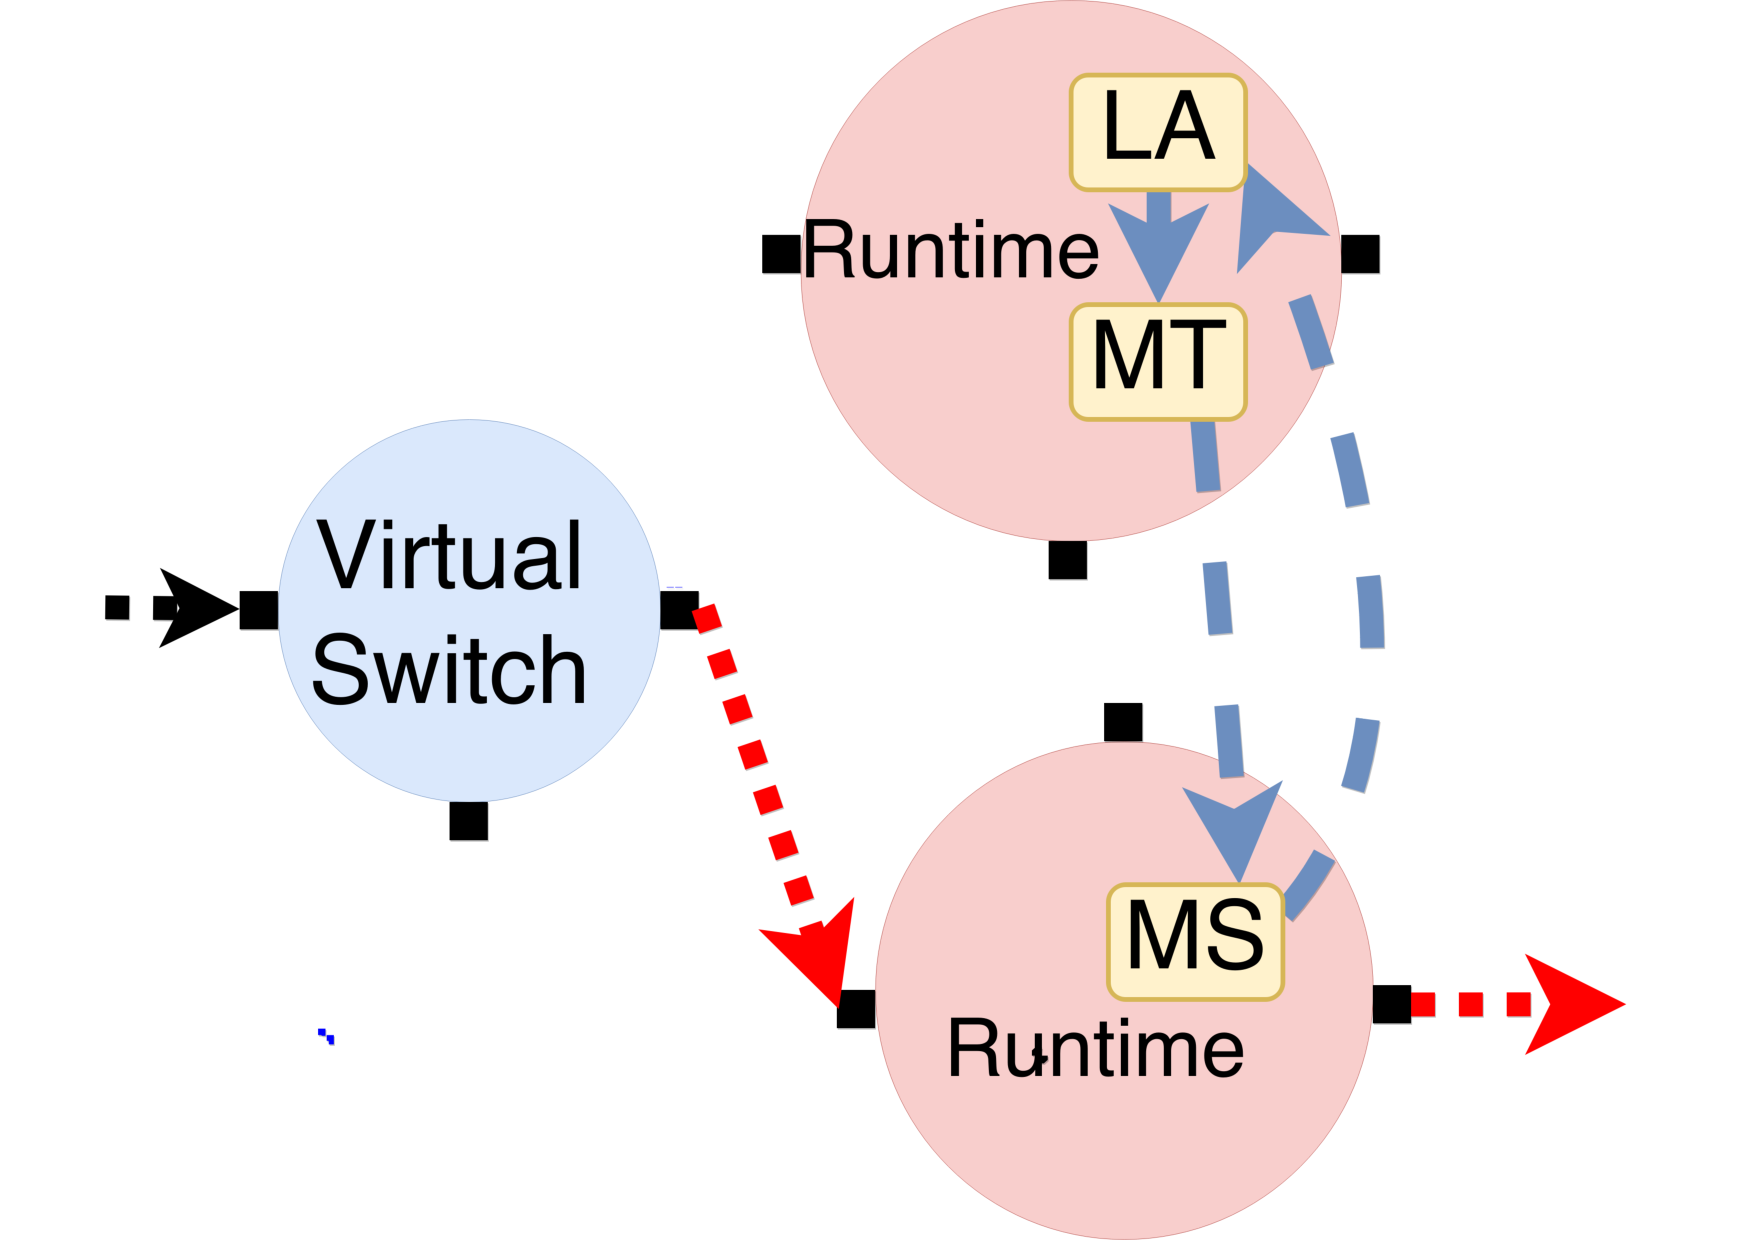
\includegraphics[width=1.1\columnwidth]{chap-nfvactor/figure/nfactor-mig1.pdf}
   \caption{1st req-rep step.}\label{fig:mig1}
  \end{subfigure}\hfill
  \begin{subfigure}[t]{0.33\linewidth}
     \centering
     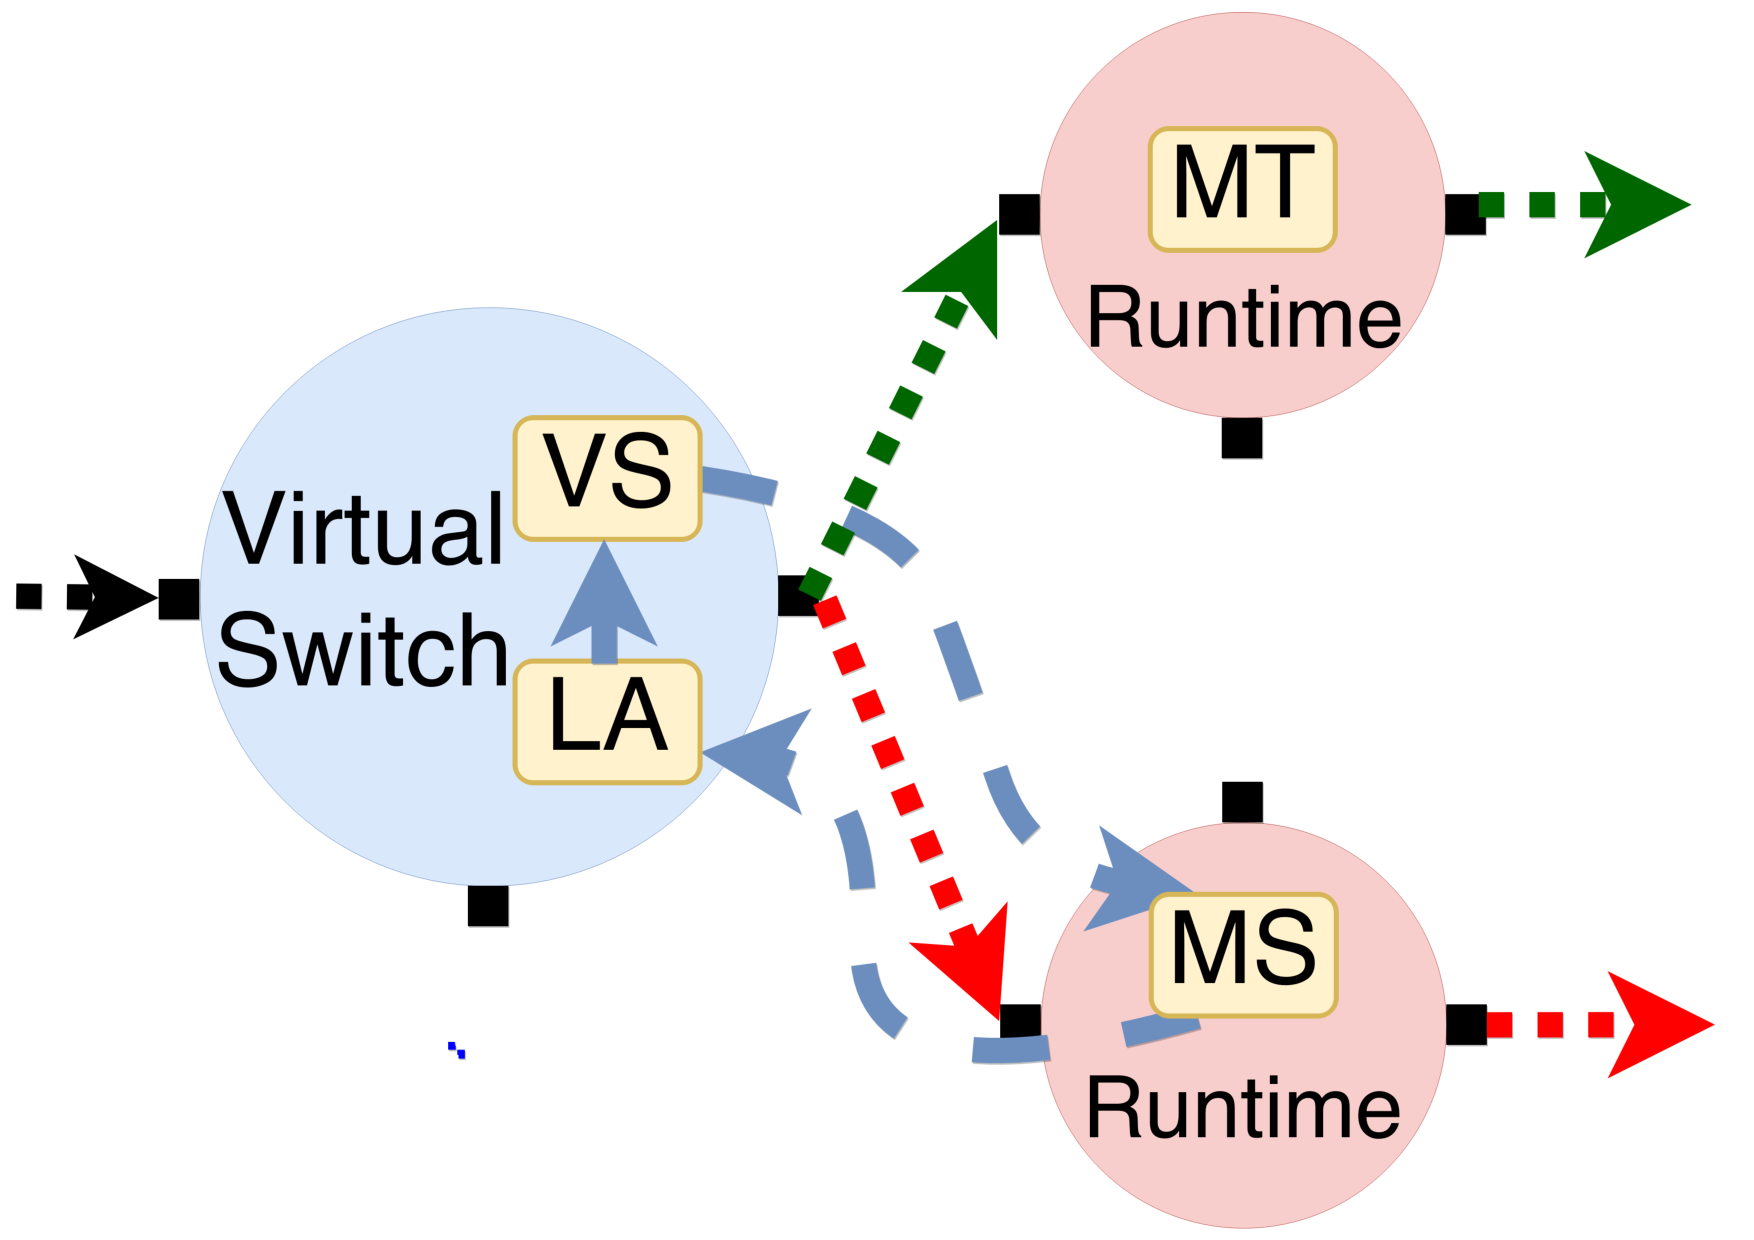
\includegraphics[width=1.1\columnwidth]{chap-nfvactor/figure/nfactor-mig2.pdf}
     \caption{2nd req-rep step.}\label{fig:mig2}
    \end{subfigure}\hfill
  \begin{subfigure}[t]{0.33\linewidth}
 \centering
   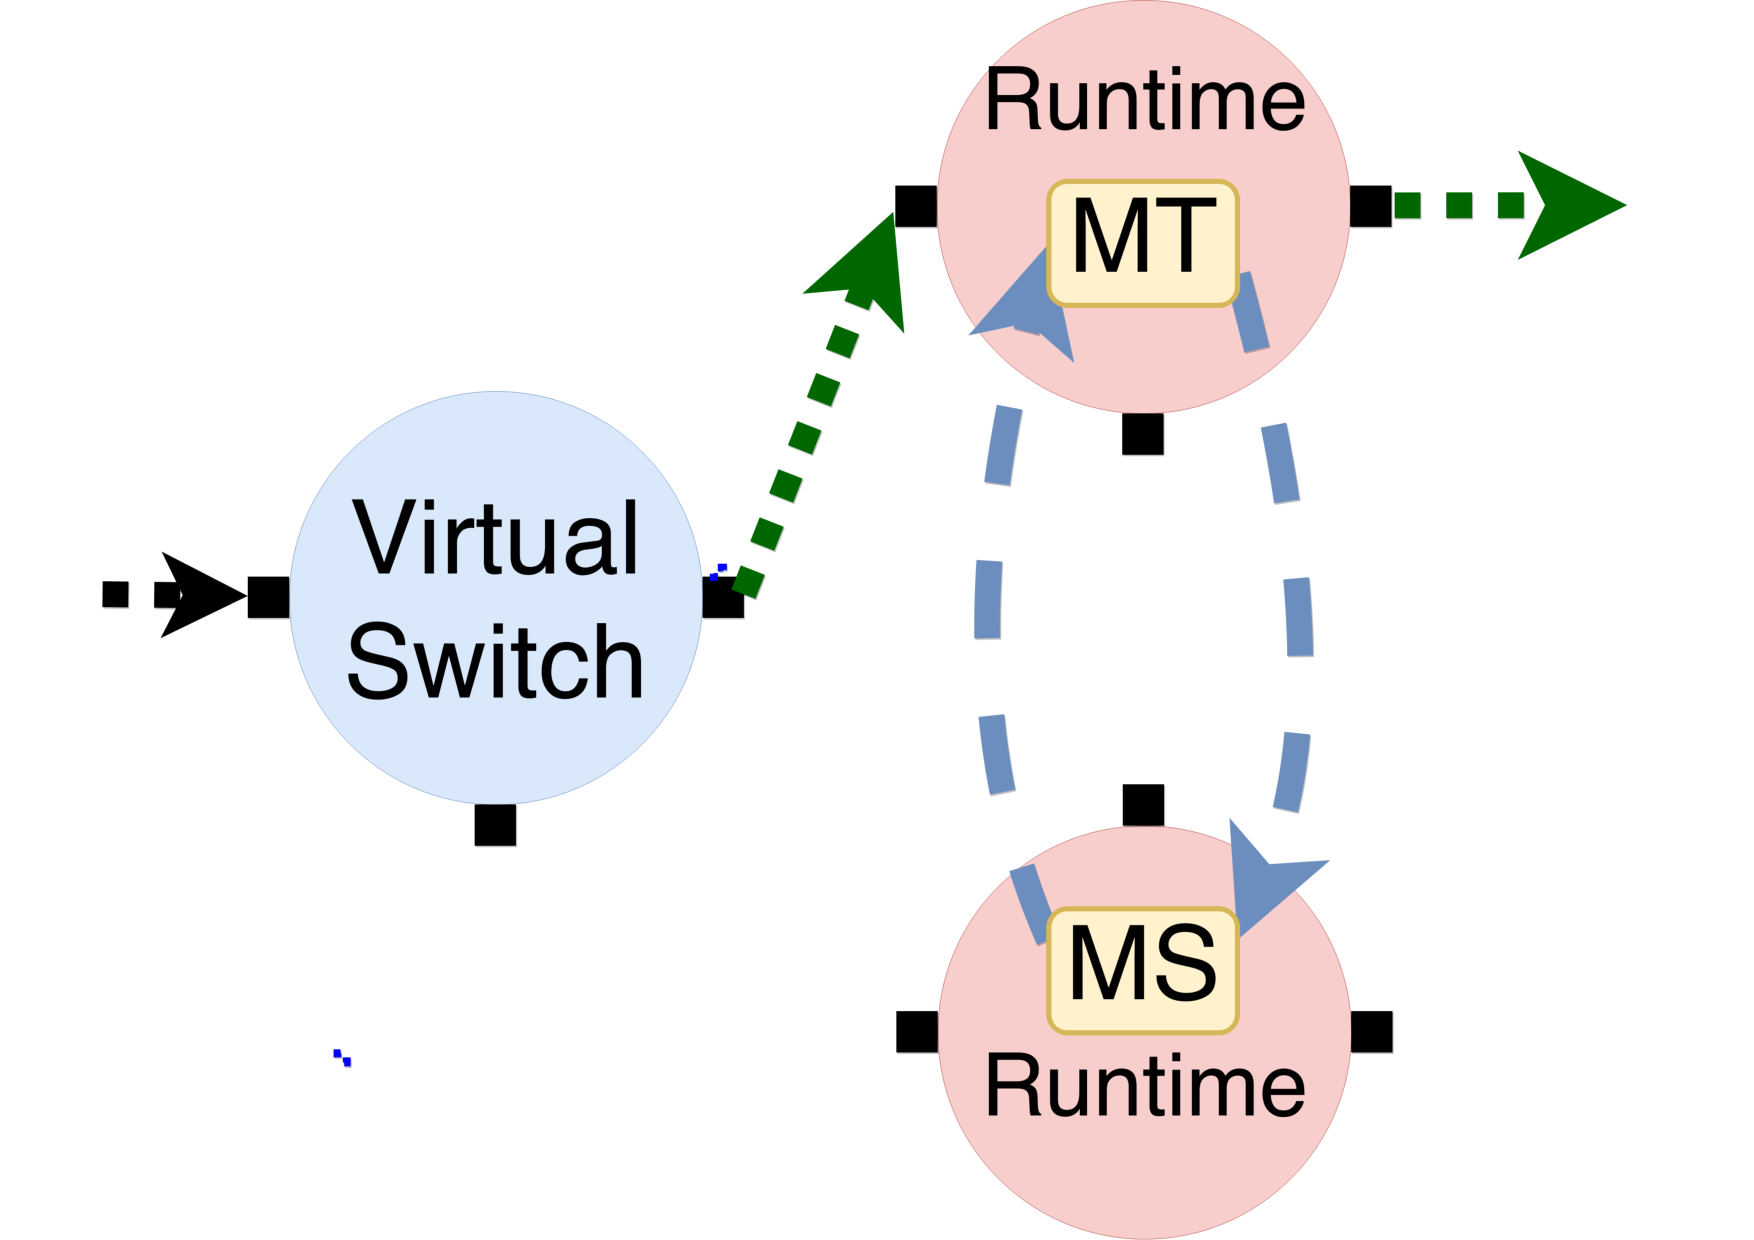
\includegraphics[width=1.1\columnwidth]{chap-nfvactor/figure/nfactor-mig3.pdf}
   \caption{3rd req-rep step.}\label{fig:mig3} \end{subfigure}\hfill
 \caption{The 3 flow migration steps: \textbf{MT} - migration target flow actor, \textbf{MS} - migration source flow actor, \textbf{LA} - liaison actor, \textbf{VS} - virtual switch actor; \textbf{dotted line} - flow packets, \textbf{dashed line} - actor messages.}
\label{fig:mig}
\end{figure}

Based on the actor model, flow migration in \nfactor~can be regarded as a transaction between a source flow actor and a target flow actor, where the source actor delivers its entire state and processing tasks to the target actor. Flow migration is successful once the target actor has completely taken over packet processing of the flow. In case of unsuccessful flow migration, the source flow actor can fall back to regular packet processing and instruct to destroy the target actor.

In \nfactor, the coordinator starts flow migration by calling $set\_migration\_target$ RPC method on a runtime, asking it to migrate a number of flows to another runtime. After receiving the ID of a migration target runtime, the flow actor starts migration by itself. The flow migration protocol used by flow actors is shown in Fig.~\ref{fig:mig}, consisting of three request-response steps. In case of request timeout, the migration source actor performs clean-up procedures and reverts to normal packet processing.

\textbf{1st req-rep step:} The source flow actor sends 5-tuple of its flow to the liaison actor on the migration target runtime. The liaison actor creates a migration target actor using the 5-tuple, and sends a response back to the migration source actor. Meanwhile, migration source actor continues to process packets as usual.

%\item
\textbf{2nd req-rep step:} The source flow actor sends the 5-tuple of its flow and the ID of the migration target runtime to the liaison actor on the virtual switch. The liaison actor uses the 5-tuple to identify the virtual switch actor in charge and notifies it to change the destination runtime to the migration target runtime. After this change, the virtual switch actor sends a response back to the source actor, and the migration target actor starts to receive packets. Instead of processing the packets, the target actor buffers all the received packets until it receives the request in the 3rd step from the source actor. The migration source actor keeps processing received flow packets until it receives the response from the virtual switch.

%\item
\textbf{3rd req-rep step:} The source flow actor sends its flow states to the migration target actor. After receiving the flow states, the migration target actor saves them, calls $flow\_migrate\_in$ (Table~\ref{table:api}) to synchronize the shared states, and immediately starts processing all the buffered packets while sending a response to the source actor. The migration source actor calls $flow\_migrate\_out$ (Table~\ref{table:api}) to synchronize the shared states and then destroys itself.

%\end{itemize}

{\em Loss Avoidance.} It is possible for our flow migration protocol to drop flow packets. However, packet drop caused by the flow migration protocol rarely happens in practice, even when concurrently migrating hundreds of thousands of flows (Sec.~\ref{sec:fmp}). We refer to this as loss-avoidance property, which is slightly weaker than the loss-free property \cite{gember2015opennf} in OpenNF.

In the 3rd step, before the request arrives at the migration target actor, the migration target actor has already received and buffered several flow packets. The buffer may overflow, causing migration target actor to drop several packets. However, our distributed flow migration finishes fast within several microseconds and such drop rarely happens in practice.
%\vspace{-1mm}

Still in the 3rd step, after the request is sent out by the source actor, it is possible for some flow packets to continue arriving at the source actor. These packets are sent out by the virtual switch actor before its destination runtime is changed in the 2nd step, but arrive later at the source actor than the response of the 2nd step. The source actor has to discard these packets because it has already sent out its flow state. ~\nfactor~minimizes the occurrence of this problem by having the virtual switch actor transmitting the response message of the 2nd step in the same network path as the flow packets, so that we rarely observe this problem in practice.
%\vspace{-1mm}

It has been a common understanding that providing good properties for flow migration would trade off the performance of flow migration \cite{gember2015opennf}. \nfactor~mitigates this trade-off using distributed, high-performance flow migration based on the actor model.
